\documentclass{article}
\usepackage{amsmath}
\usepackage[margin=1in]{geometry}
\usepackage{amsfonts}
\usepackage{hyperref}
\usepackage{graphicx}
\usepackage{amssymb}


\begin{document}
	
	\title{Modulo}
	\author{Andy Chong Sam}	
	\maketitle	
	
\section {Remainder Quotient Formula}

\par\noindent When performing an integer division we can document a quotient (q) and a remainder (r). In this document we will use the following notation to denote each:

\begin{flalign*}
	a/b=q \\
	a\mod b = r 
\end{flalign*}

\par\noindent  Given a dividend \(a\), and a divisor \(b\) that results in a quotient \(q\) and a remainder \(r\) , we can derive the following expression:

\begin{flalign}
	a = bq + r
\end{flalign}
	
\par\noindent  Consider a simple integer division of 25 divided by 11. Since \(25/11=2\) and \(25\mod11=3\), all pieces of the operation can be encapsulated as: \(25=(11)(2) + 3\). Expression (1) can be used to demonstrate various properties in modular arithmetic.

\section {Modular Arithmetic}

\subsection{Overview}

\par\noindent A straightforward interpretation of the modulo operation (mod) is that its output is the remainder of the division between two integers. A cyclical pattern is observed by varying x in \(x \mod s\), when s is left constant.
\newline 	
\par\noindent For \(x \mod 1\), the set of all possible outcomes is \{0\}.

\par\noindent For \(x \mod 2\), the set of all possible outcomes is \{0,1\}.

\par\noindent For \(x \mod 5\), the set of all possible outcomes is \{0,1,2,3,4\}.

\subsection{Negative Dividends}

\par When the dividend is negative, the results are less intuitive. For example: \(-11\mod3=1\). One way to visualize this outcome is by imagining a number line with an emphasis on the range of mod 3: \(\{0,1,2\}\)
\newpage
	\begin{center}
	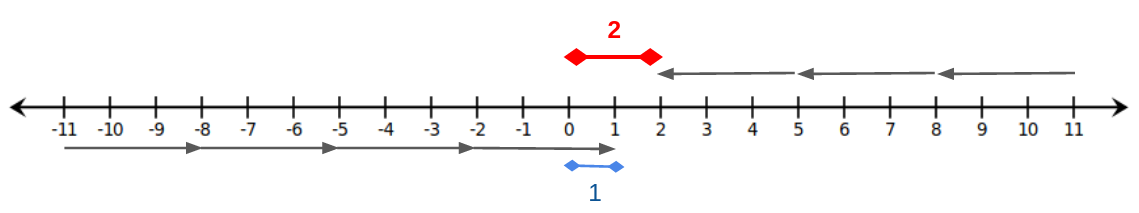
\includegraphics[width=11cm]{mod-num-line.png}
\end{center}
\begin{minipage}[c]{.45\linewidth}


		In the case of \(-11 \mod 3\) we can see that there are 4 skips needed to enter the modulo range. The distance between where the last skip lands and 0 is the modulo. In this case, this distance is 1.




\end{minipage}
\begin{minipage}[c]{.45\linewidth}
	

		In the case of \(11 \mod 3\) we can see that there are 3 skips needed to enter the modulo range. The distance between where the last skip lands and 0 is the modulo. In this case, this distance is 2.


\end{minipage}
\linebreak
\linebreak
\par\noindent For the operation \(a \mod b\) and if a is negative, then we can calculate the modulo using the following expression:

\begin{flalign}
	a + \lvert \lfloor \frac{a}{b} \rfloor \rvert(b) + b
\end{flalign} 

\subsection{Modular Addition}

\par\noindent The property of modular addition is as follows:

\begin{flalign}
	(a+b)\mod c = ((a\mod c )+ (b\mod c))\mod c
\end{flalign} 

\par\noindent This relationship can be derived by using expression (1). Recall that if a is divisible by c, and b is divisible by c, then a+b is divisible by c. We first start by restating a + b:

\begin{flalign*}
a = cq_{1} + r_{1} \therefore a \mod c = r_{1}\\
b = cq_{2} + r_{2} \therefore b \mod c = r_{2}\\
a+b = (cq_{1} + r_{1} + cq_{2} + r_{2}) \\
a+b = c(q_{1} + q_{2}) + r_{1} + r_{2}
\end{flalign*} 

\par\noindent Plugging the above result back into \((a+b) \mod c\) we get:

\begin{flalign*}
	(c(q_{1} + q_{2}) + r_{1} + r_{2}) \mod c
\end{flalign*}

\par\noindent We can apply the following rule to simplify the above expression. If we have an operation \(a \mod b\), then we know that adding a multiple of b (say kb), will result in the same modulo value: \((a + kb) \mod b = a\mod b\). We can now simplify further:

\begin{flalign*}
	(c(q_{1} + q_{2}) + r_{1} + r_{2}) \mod c \\
	= (r_{1} + r_{2}) \mod c
\end{flalign*}

\par\noindent On the right hand side of expression (3) we can simplify further, using:

\begin{flalign*}
	a = cq_{1} + r_{1} \therefore a \mod c = r_{1}\\
	b = cq_{2} + r_{2} \therefore b \mod c = r_{2}\\
\end{flalign*}

\par\noindent So the right hand side becomes \( (r_{1} + r_{2}) \mod c\) as well.

\subsection{Modular Multiplication}

\par\noindent The property of modular multiplication is as follows:

\begin{flalign}
	(ab)\mod c= ( (a\mod c) \;\; (b\mod c)) \mod c
\end{flalign}

\par\noindent This can be derived in a way similar to modular addition. The left hand side can be rewritten like so:

\begin{flalign*}
	((cq_{1} + r_{1})(cq_{2} + r_{2})) \mod c \\
	= (  c^{2}   q_{1}  q_{2} + cq_{1}r_{2} + cq_{2}r_{1} + r_{1}r_{2}) \mod c \\
	= (c(cq_{1}q_{2} + q_{1}r_{2} + q_{2}r_{1}) + r_{1}r_{2}) \mod c
\end{flalign*}

\par\noindent Since \(c(cq_{1}q_{2} + q_{1}r_{2} + q_{2}r_{1})\) is a multiple of c, we are left with:

\begin{flalign*}
	(r_{1}r_{2})\mod c
\end{flalign*}

\par\noindent On to the right hand side of expression (4), using:

\begin{flalign*}
	a = cq_{1} + r_{1} \therefore a \mod c = r_{1}\\
	b = cq_{2} + r_{2} \therefore b \mod c = r_{2}\\
\end{flalign*}

\par\noindent We see that the right hand side of expression (4) becomes:

\begin{flalign*}
	(r_{1}r_{2})\mod c
\end{flalign*}

\subsection{Modular Exponentiation}

\par\noindent Modular exponentiation takes the form of evaluation a problem like \(a^{x} \mod b\). The challenge here is that \(a^{x}\) could easily become a very large number, causing errors on calculators. A commonly used technique to overcome this problem is known as "fast modular exponentiation" and it involves restating x using base-2.

\par\noindent Suppose we are trying to evaluate \(7^{15} \mod 17\). The first step is to translate the exponent into base-2. The number 15 thus becomes \( (1111)_{2} \). We can expand this base-2 number with each term representing the binary symbol \{0,1\} times 2 raised to the power of the place value it appears in:

\begin{flalign*}
	15 = (1)(2)^{3} + (1)(2)^{2} + (1)(2)^{1} + (1)(2)^{0}
\end{flalign*}

\par\noindent With this expansion in mind, we can restate the original problem like so:

\begin{flalign*}
	7^{15} \mod 17 \\
	= (7^{(1)2^{3} + (1)2^{2} + (1)2^{1} + (1)2^{0} }) \mod 17 \\
	= (7^{8 + 4 + 2 + 1 }) \mod 17 \\
\end{flalign*}

\par\noindent Finally, we can apply the algebraic rule of exponents and the property of modular multiplication:

\begin{flalign*}
	(7^{8 + 4 + 2 + 1 }) \mod 17 \\
	= ((7^{8} \mod 17) \;\;\;(7^{4} \mod 17)\;\;\;(7^{2} \mod 17)\;\;\;(7^{1} \mod 17)) \mod 17
\end{flalign*}

\par \noindent We have now broken the problem into individual components, thus making calculations easier and reducing the likelikhood of overflow errors.

\section{Euclidean Algorithm}

\subsection{GCD and Algorithm Steps}
\par\noindent The Greatest Common Divisor (GCD) is the largest common divisor for a set of numbers. 
\newline
\par\noindent The Euclidean Algorithm outlines a series of steps that can be followed to arrive at the GCD for two integers (say a and b). We start by taking the larger of the two numbers, let's say a, and rewrite it using the remainder quotient formula: \(a = bq_{1} + r_{1}\). We will then evaluate \(b = r_{1}q_{2} + r_{2} \). We could potentially evaluate \(r_{1}= r_{2}q_{3} + r_{3} \). 
\newline

\par\noindent We could encapsulate this recursive operation as \(E(s,t) \rightarrow s = tq_{n} + r_{n}\). We stop when s or t becomes 0, and the non-zero value will be the GCD.
\newline
\newline
\framebox{
	\parbox{\linewidth}{
\par\noindent \textbf{Ex. 1} Evaluate \(gcd(93,42)\)
\newline

	\begin{flalign*}
	E(93,42) \rightarrow 93 = (2)(42) + 9 \\
	E(42,9) \rightarrow 42 = (4)(9) + 6 \\
	E(9,6) \rightarrow 9 = (6)(1) + 3 \\ 	
	E(6,3) \rightarrow 6= (3)(2) + 0 \\
	E(3,0)	
\end{flalign*}

\par\noindent \textbf{Solution:}  \(gcd(93,42) = 3\)	
	}
}
\newline
\newline
\newline
\framebox{
	\parbox{\linewidth}{
\par\noindent \textbf{Ex. 2}  Evaluate \(gcd(4278,8602)\)

\begin{flalign*}
	E(8602,4278) \rightarrow 8602 = (4278)(2) + 96 \\
	E(4278,96) \rightarrow 4278 = (46)(93) + 0 \\
	E(46,0)
\end{flalign*}	
\newline
\newline
\par\noindent So \(gcd(4278,8602) = 46\)
}
}

\newpage
\subsection{Bézout's Lemma}

\par\noindent There are integers x and y such that \(gcd(a,b) = xa + yb\). Matrices with elementary row operations can be used to find \(x\) and \(y\). We will demonstrate the algorithm using the two examples above. 
\newline


\framebox{
	\parbox{\linewidth}{
		\par\noindent \textbf{Ex. 3} Our claim is that there are integers x and y such that \(gcd(93,42) = 93x + 42y\). 
		\newline
		\newline
		\begin{minipage}[c]{.20\linewidth}	
			\begin{center}
				\textbf{State Matrix}
			\end{center}			
		\end{minipage}
		\begin{minipage}[c]{.40\linewidth}
			
			\begin{center}
				\textbf{Division}
			\end{center}
			
		\end{minipage}
		\begin{minipage}[c]{.33\linewidth}
			\textbf{Elementary Row Operation}
		\end{minipage}
		
		\begin{minipage}[c]{.20\linewidth}	
			\begin{center}
				$\begin{bmatrix}
					1 & 0 & 93 \\
					0 & 1 & 42
				\end{bmatrix}$ 
			\end{center}			
		\end{minipage}
		\begin{minipage}[c]{.40\linewidth}
			\begin{flalign*}
				93/42 = 2 \\
				93 \mod 42 = 9 	
			\end{flalign*}	
			
		\end{minipage}
		\begin{minipage}[c]{.33\linewidth}
			\begin{flalign*}
				R_{1} - 2R_{2} \rightarrow R_{1}
			\end{flalign*}	
			
		\end{minipage}
		
		\begin{minipage}[c]{.20\linewidth}	
			\begin{center}
				$\begin{bmatrix}
					1 & -2 & 9 \\
					0 & 1 & 42
				\end{bmatrix}$ 
			\end{center}			
		\end{minipage}
		\begin{minipage}[c]{.40\linewidth}
			\begin{flalign*}
				42/9 = 4 \\
				42 \mod 92 = 6 	
			\end{flalign*}	
			
		\end{minipage}
		\begin{minipage}[c]{.33\linewidth}
			\begin{flalign*}
				R_{2} - 4R_{21} \rightarrow R_{2}
			\end{flalign*}		
		\end{minipage}
		
		\begin{minipage}[c]{.20\linewidth}	
			\begin{center}
				$\begin{bmatrix}
					1 & -2 & 9 \\
					-4 & 9 & 6
				\end{bmatrix}$ 
			\end{center}			
		\end{minipage}
		\begin{minipage}[c]{.40\linewidth}
			
			\begin{flalign*}
				9/6 = 1 \\
				9 \mod 6 = 3 	
			\end{flalign*}	
			
		\end{minipage}
		\begin{minipage}[c]{.33\linewidth}
			\begin{flalign*}
				R_{1} - R_{2} \rightarrow R_{1}
			\end{flalign*}		
		\end{minipage}
		
		\begin{minipage}[c]{.20\linewidth}	
			\begin{center}
				$\begin{bmatrix}
					5 & -11 & 3 \\
					-4 & 9 & 6
				\end{bmatrix}$ 
			\end{center}			
		\end{minipage}
		\begin{minipage}[c]{.40\linewidth}
			\begin{flalign*}
				6/3 = 2 \\
				6 \mod 3 = 0 	
			\end{flalign*}	
		\end{minipage}
		\begin{minipage}[c]{.33\linewidth}
			The stopping condition, that \(6 \mod 3 = 0 \), has been reached. 
		\end{minipage}
		\newline
		\newline
		
		\par\noindent \textbf{Solution:} So \(x=5\) and \(y=-11\). We can verify this: \((93)(5) + (42)(-11) = 3\).
}

}
\newline
\newline
\newline

\framebox{
	\parbox{\linewidth}
	{
\par\noindent \textbf{Ex. 4} Our claim is that there are integers x and y such that \(gcd(4278,8602) = 8602x + 4278y\). 
\newline
\newline
\begin{minipage}[c]{.20\linewidth}	
	\begin{center}
		\textbf{State Matrix}
	\end{center}			
\end{minipage}
\begin{minipage}[c]{.40\linewidth}
	
	\begin{center}
		\textbf{Division}
	\end{center}
	
\end{minipage}
\begin{minipage}[c]{.33\linewidth}
	\textbf{Elementary Row Operation}
\end{minipage}

\begin{minipage}[c]{.20\linewidth}	
	\begin{center}
		$\begin{bmatrix}
			1 & 0 & 8602 \\
			0 & 1 & 4278
		\end{bmatrix}$ 
	\end{center}			
\end{minipage}
\begin{minipage}[c]{.40\linewidth}
	
	\begin{flalign*}
		8602/4278 = 2 \\
		8602 \mod 4278 = 46	
	\end{flalign*}	
	
\end{minipage}
\begin{minipage}[c]{.33\linewidth}
	\begin{flalign*}
		R_{1} - 2R_{2} \rightarrow R_{1}
	\end{flalign*}		
\end{minipage}

\begin{minipage}[c]{.20\linewidth}	
	\begin{center}
		$\begin{bmatrix}
			1 & -2 & 46 \\
			0 & 1 & 4278
		\end{bmatrix}$ 
	\end{center}			
\end{minipage}
\begin{minipage}[c]{.40\linewidth}
	
	\begin{flalign*}
		4278/46 = 93 \\
		4278 \mod 46 =0	
	\end{flalign*}	
	
\end{minipage}
\begin{minipage}[c]{.33\linewidth}
	\par\noindent The stopping condition has been reached.		
\end{minipage}
\newline
\par\noindent \textbf{Solution:} So \(x=1\) and \(y=-2\). We can verify this: \( (8602)(1) + (4278)(-2) = 46\)	
}
}
\newline
\newline
\newline

\section{Congruence}

\subsection{Overview}
\par\noindent The statement \(a \equiv b \mod n\), is another way of stating \(a \mod n = b \mod n\). For example, \(7 \equiv 12 \mod 5\) is a true statement, since \(7 \mod 5 = 2\) and \( 12 \mod 5 = 2\). We also find that \(17 \mod 5 = 2\). These 3 integers belong to the same Congruence Class for mod 5.
\newline
\newline
Referring back to section 2.1, we know that the only possible outcomes of any integer x mod 5 is \{0,1,2,3,4\}. Therefore there are 5 different congruence classes for mod 5.

\subsection{Solving Congruence Problems}

\par\noindent Several strategies can be applied to solve the problems of the form \(ax \equiv b (\mod n)\). For the next few examples, we will use the following five propositions:
\newline
\newline
\par\noindent \textbf{(p1)} If d divides n and we have \(ad \equiv bd (\mod n)\), we can simplify this to \(a \equiv b (\mod \frac{n}{d})\)
\newline
\par\noindent \textbf{(p2)} If \(gcd(a,n) = 1\) and we have \(ad \equiv bd (\mod n)\), we can simplify this to \(a \equiv b (\mod n)\)
\newline
\par\noindent \textbf{(p3)} There is a solution to \(ax \equiv b (\mod n)\) if \(gcd(a,b) | n\)
\newline
\par\noindent \textbf{(p4)} For \(a\bar{a} = 1 (\mod n)\), the inverse \(\bar{a}\) exists if \(gcd(a,n) = 1\)
\newline
\par\noindent \textbf{(p5)} For \(ax \equiv b (\mod n)\) where multiple solutions exist, the spread between solutions is \(\frac{n}{gcd(a,n)}\)
\newline
\newline
\par\noindent Sometimes the solution to a problem is trivial and involves only algebra, consider the following two problems:
\newline

\framebox{
	\parbox{\linewidth}{
\par \noindent \textbf{Ex. 5} Solve \(8x \equiv 16(\mod 5)\)  :
\newline
\par\noindent First, we observe that \(gcd(8,5) = 1\). We can divide both sides of the congruence by 8 (applying \textbf{p2}).

\begin{flalign*}
	x \equiv 2 (\mod 5)	\\
	\text{To verify our solution:}\\
	(8)(2) \equiv 16 (\mod 5)\\
	16 \equiv 16 (\mod5)
\end{flalign*}
\par\noindent \textbf{Solution:} \( x \equiv 2 (\mod 5)\) 
}
}
\newline
\newline

\framebox{
	\parbox{\linewidth}{
\par \noindent \textbf{Ex. 6} Solve \(2x \equiv 8(\mod 3)\)  :
\newline
\par\noindent First, we observe that \(gcd(2,3) = 1\). We can divide both sides of the congruence by 2 (applying \textbf{p2}).
\newline
\begin{flalign*}
	x \equiv 4 (\mod 3) \\
	\text{To verify our solution:}\\
	(2)(4) \equiv 8 (\mod 3)\\
	8 \equiv 8 (\mod 3)
\end{flalign*}
\par\noindent \textbf{Solution:}\(4x \equiv (\mod 3)\)	
}
}
\newpage
\par \noindent In some cases, algebra by itself will not work as the division on both sides of the congruence would not produce an integer. For these cases, we can first verify if a solution exists, and determine if a and n are coprime. If a and n are coprime, we we can use the modulo multiplicative inverse.
\newline
\par\noindent For a problem \(ax \equiv b(\mod n)\), we first check if \(gcd(a,n) = 1\). If so, we we can evaulate \( a\bar{a} \equiv 1 (\mod n)\). Once we determine the value of \(\bar{a}\). We can multiply both sides of the original congruence by \( \bar{a}\):

\begin{flalign*}
	a\bar{a}x \equiv \bar{a}b (\mod n) \\
	x \equiv \bar{a}b (\mod n)
\end{flalign*}

\par\noindent Let's clarify what happens to the dropped coefficient on the left. The expression \(a\bar{a}x \equiv \bar{a}b (\mod n) \) can be restated as \(a\bar{a}x \mod n = \bar{a}b\mod n\). 
\newline
\par\noindent On the left hand side, \(\bar{a}\) is an integer, that when multiplied by \(ax\) and divided by n,  produces a remainder of 1: \(a\bar{a}x \mod n = 1\). This is functionally equivalent to saying \((1)(x) \mod n = 1\). We can now rewrite the left hand side:

\begin{flalign*}
		a\bar{a}x \mod n = \bar{a}b \mod n \\
		(1)x \mod n = \bar{a}b \mod n \\
			x \equiv \bar{a}b (\mod n)
\end{flalign*}

\par\noindent Let's consider a few examples:
\newline
\newline
\framebox{
	\parbox{\linewidth}{
\par\noindent\textbf{Ex. 7} Solve \(3x \equiv 7 (\mod 11)\)
\newline
\par\noindent We first determine that gcd(3,11)=1, so the method can be applied. Since \(1 | 11\), an inverse \(\bar{a}\) exists. After some tests, we determine that \(\bar{a}\) is 4.
\begin{flalign*}
	(3)(4) \mod 11 = 1 \\
	\therefore \bar{a} = 4,
\end{flalign*}
\par\noindent We can now use \(\bar{a}\) to solve the original problem:
\begin{flalign*}
	4x \equiv (4)(7) (\mod 11) \\
	x \equiv 28 (\mod 11)	
\end{flalign*}
\par\noindent We can improve the answer by reporting the smallest positive value. The spread is 11, so \(x \equiv 6 (\mod 11)\) is the best answer. Finally, we can do a quick verification:
\begin{flalign*}
	(3)(6) \mod 11 \\
	= 18 \mod 11 \\
	= 7	
\end{flalign*}	
\par\noindent Solution: \(x \equiv 6 (\mod 11)\)
}
}
\newpage
\framebox{
	\parbox{\linewidth}{
\par\noindent\textbf{Ex. 8} Solve \(21x \equiv 14(\mod 91)\)
\newline
\par\noindent We notice that \(gcd(21,91) = 7\), so at first glance the inverse technique might not work. However, we can simplify the congruence by dividing both sides by 7, and also divide 91 by 7 (Applying \textbf{p1}):

\begin{flalign*}
	21x \equiv 14(\mod 91) \\
	3x \equiv 2(\mod 13) \\
\end{flalign*}

\par\noindent We can now apply the technique. We find \(gcd(3,13) = 1\), and since \( 1 | 13\) an inverse exists. After testing some numbers we find:

\begin{flalign*}
	(3)(9) \mod 13 = 1 \\
	\therefore \bar{a} = 9
\end{flalign*}

\par\noindent We can now use \(\bar{a}\) to solve the original problem:

\begin{flalign*}
	(9)(3)x \equiv (9)(2)(\mod 13) \\
	x \equiv 18 (\mod 13)
\end{flalign*}

\par\noindent Like the previous problem, we can report a slightly better answer by using the spread, which is 13, leaving us with \(x \equiv 5 (\mod 13)\). We can verify the answer:

\begin{flalign*}
	(21)(5) \mod 91 \\
	= 105 \mod 91 \\
	= 14
\end{flalign*}

\par\noindent Solution: \(x \equiv 5 (\mod 13)\)
}
}
\newline

\framebox{
	\parbox{\linewidth}{

\par\noindent\textbf{Ex. 9} Solve \(19x \equiv 4 (\mod 141) \)
\newline
\par\noindent Since \(gcd(19,141) = 1\) and \( 1 | 141\), the inverse technique can be applied. First we find \(\bar{a}\):

\begin{flalign*}
	(19)(52) \mod 141 = 1 \\
	\therefore \bar{a} = 52	
\end{flalign*}

\par\noindent We can now use \(\bar{a}\) to solve the original problem:

\begin{flalign*}
	(52)(19)x \equiv (52)(4) ( \mod 141) \\
	x \equiv 208 (\mod 141)
\end{flalign*}

\par\noindent Since the spread is 141, a better answer to report would be \( x \equiv 67 (\mod141)\). Let's verify the result:

\begin{flalign*}
	(19)(67) \mod 141 \\ 
	=1273 \mod 141 \\
	=4
\end{flalign*}

\par\noindent Solution: \(x \equiv 67 (\mod 141)\)
}
}
\section {The Chinese Remainder Theorem}

\par\noindent The Chinese remainder Theorem outlines an algorithm that can be used to solve a system of congruences. The steps are illustrated below using a system of three congruences. Suppose we want to solve the following:

\begin{flalign*}
	x \equiv b_{1} (\mod c_{1}) \\
	x \equiv b_{2} (\mod c_{2}) \\
	x \equiv b_{3} (\mod c_{3})
\end{flalign*}

\par\noindent The theorem can be used if \(c_{1}, c_{2}, c_{3}\) are coprime. We first calculate \(N = (c_{1})(c_{2})(c_{3})\). We then setup the following table:
\newline
\begin{center}
	\begin{tabular}{||c c c c||} 
		\hline
		\(b_{i} \)& \(N_{i}\) & \(\bar{a}\) & \(b_{i}N_{i}a_{i} \) \\ [0.5ex] 
		\hline\hline
		\(b_{1} \)& \(N_{1}=n_{2}n_{3}\) & \(\bar{a}_{1}\)& \vline \;\;\(b_{1}N_{1}a_{1} \) \\ 
		\hline
		\(b_{2} \) & \(N_{2}=n_{1}n_{3}\) &\(\bar{a}_{2}\) & \vline \;\;\(b_{2}N_{2}a_{2} \) \\
		\hline
		\(b_{3} \) & \(N_{3}=n_{1}n_{2}\) & \(\bar{a}_{3}\)& \vline \;\;\(b_{3}N_{3}a_{3} \) \\
		\hline
	\end{tabular}
\end{center}
\par\noindent The column \(N_{i}\) represents the calculation \(N_{i} = \frac{N}{n_{i}}\). The column \( \bar{a} \) is the solution to \(\bar{a}\) in \( N_{i}\bar{a}_{i} \equiv 1 (\mod c_{i})  \). The solution to the system is the sum of the last column mod N:

\begin{flalign*}
 (\sum_{i=1}^{3} b_{i}N_{i}a_{i}) \mod N
\end{flalign*}


\newpage

\par\noindent Here is an example of the algorithm in action. 
\newline
\newline
\framebox{
	\parbox{\linewidth}{
\par\noindent \textbf{Ex. 10} Suppose that there is a group of students, and the instructor has a choice to group everyone into teams of 3, 4, or 5. If groups of 3 are created, there will be 2 students unassigned students left over. If groups of 4 are made, then there will be 3 students left over, and in the case of groups of 5, then there will be 1 student left over. We want to find a class size that would result in the above outcomes.
\newline
\par\noindent The problem can be summarized into the following system of congruences:
\begin{flalign*}
	x \equiv 3 (\mod 4) \\
	x \equiv 1 (\mod 5) \\
	x \equiv 2 (\mod 3) \\
\end{flalign*}
\par\noindent From the initial setup, we can see that \(N=(4)(5)(3)=60\). We can start to fill in some of the table details:
\begin{center}
	\begin{tabular}{||c c c c||} 
		\hline
		\(b_{i} \)& \(N_{i}\) & \(\bar{a}\) & \(b_{i}N_{i}a_{i} \) \\ [0.5ex] 
		\hline\hline
		3 & 15 & \(\bar{a}_{1}\)& \vline \;\;\(b_{1}N_{1}a_{1} \) \\ 
		\hline
		1 & 12 &\(\bar{a}_{2}\) & \vline \;\;\(b_{2}N_{2}a_{2} \) \\
		\hline
		2 & 20 & \(\bar{a}_{3}\)& \vline \;\;\(b_{3}N_{3}a_{3} \) \\
		\hline
	\end{tabular}
\end{center}
\par\noindent The next step is to figure out \(\bar{a}_{i}\). After some trial and error, we determine the following:
\begin{flalign*}
	(15)(3) \equiv 1 (\mod 15) \therefore \bar{a}_{1} = 3 \\
	(12)(3) \equiv 1 (\mod 12) \therefore \bar{a}_{2} = 3 \\
	(20)(2) \equiv 1 (\mod 20) \therefore \bar{a}_{3} = 2 \\ 
\end{flalign*}
\par\noindent  We can now complete the table:
\begin{center}
	\begin{tabular}{||c c c c||} 
		\hline
		\(b_{i} \)& \(N_{i}\) & \(\bar{a}\) & \(b_{i}N_{i}a_{i} \) \\ [0.5ex] 
		\hline\hline
		3 & 15 & 3 & \vline \;\;135 \\ 
		\hline
		1 & 12 & 3 & \vline \;\;\;\;36 \\
		\hline
		2 & 20 & 2 & \vline \;\;\;\;80 \\
		\hline
	\end{tabular}
\end{center}
\par\noindent  The sum of the last column is 251. At this point, we have \(x \equiv 251 (\mod 60)\). Since the spread is 60, the best reportable answer is \(x \equiv 11 (\mod 60)\). We can verify this result:

\begin{flalign*}
	11 \mod 4 = 3 \;\;\;\;\;\;\; 11 \mod 5 = 1 \;\;\;\;\;\;\; 11 \mod 3 = 2 
\end{flalign*}

\par\noindent So a class size of 15 meets the criteria, with 3 students left if groups of 4 are made, 1 student left if groups of 5 are made, and 2 left with groups of 3.

}
}
\newline

\newpage


\framebox{
	\parbox{\linewidth}{
\par\noindent \textbf{Ex. 11} Here is an additional example. solve the following system:		
		
		\begin{flalign*}
			x \equiv 3 (\mod 5) \\
			x \equiv 1 (\mod 7) \\
			x \equiv 6 (\mod 8) \\
		\end{flalign*}
		
		\par\noindent First, we determine that \(N=(5)(7)(8)=280\). We can partially fill our table:
		
		\begin{center}
			\begin{tabular}{||c c c c||} 
				\hline
				\(b_{i} \)& \(N_{i}\) & \(\bar{a}\) & \(b_{i}N_{i}a_{i} \) \\ [0.5ex] 
				\hline\hline
				3 & 56 & \(\bar{a}_{1}\)& \vline \;\;\(b_{1}N_{1}a_{1} \) \\ 
				\hline
				1 & 40 &\(\bar{a}_{2}\) & \vline \;\;\(b_{2}N_{2}a_{2} \) \\
				\hline
				6 & 35 & \(\bar{a}_{3}\)& \vline \;\;\(b_{3}N_{3}a_{3} \) \\
				\hline
			\end{tabular}
		\end{center}
		
		\par\noindent The next step is to figure out \(\bar{a}_{i}\). After some trial and error, we determine the following:
		
		\begin{flalign*}
			(56)(1) \equiv 1 (\mod 8) \therefore \bar{a}_{1} = 1\\
			(40)(5) \equiv 1 (\mod 7) \therefore \bar{a}_{2} = 3\\
			(40)(5) \equiv 1 (\mod 7) \therefore \bar{a}_{3} = 3\\
		\end{flalign*}
		
		\par\noindent We complete the table:
		
		\begin{center}
			\begin{tabular}{||c c c c||} 
				\hline
				\(b_{i} \)& \(N_{i}\) & \(\bar{a}\) & \(b_{i}N_{i}a_{i} \) \\ [0.5ex] 
				\hline\hline
				3 & 56 & 1 & \vline \;\; 168 \\ 
				\hline
				1 & 40 & 3 & \vline \;\; 120 \\
				\hline
				6 & 35 & 3 & \vline \;\; 630 \\
				\hline
			\end{tabular}
		\end{center}
		
		\par\noindent Given the sum of the last column, we have \(x \equiv 918 (\mod 280)\). Since the spread is 280, the best reportable answer is \(x \equiv 78 (\mod 280)\)
		
	}
}

\end{document}

